
\chapter{Tri par insertion}
\section{Fonctionnement de l'algorithme}

Le tri par insertion est un algorithme de tri simple qui fonctionne de manière similaire à la façon dont nous trions les cartes à jouer entre mains. 
\par
Le tableau est virtuellement divisé en une partie triée et une partie non triée. Les valeurs de la partie non triée sont sélectionnées et placées à la bonne position dans la partie triée.
\par
Les étapes sur la façon dont cet algorithme fonctionne se résume comme suit :
\begin{itemize}
\item Si c'est le premier élément, il est déjà trié.
\item Choisissez l'élément suivant.
\item Comparez avec tous les éléments de la sous-liste triée.
\item Décalez tous les éléments de la sous-liste triée qui sont supérieurs à la valeur à trier vers la droite, puis insérez la valeur.
\item Répétez jusqu'à ce que la liste soit triée.
\end{itemize}
\\
\begin{figure}[H]
    \centering
        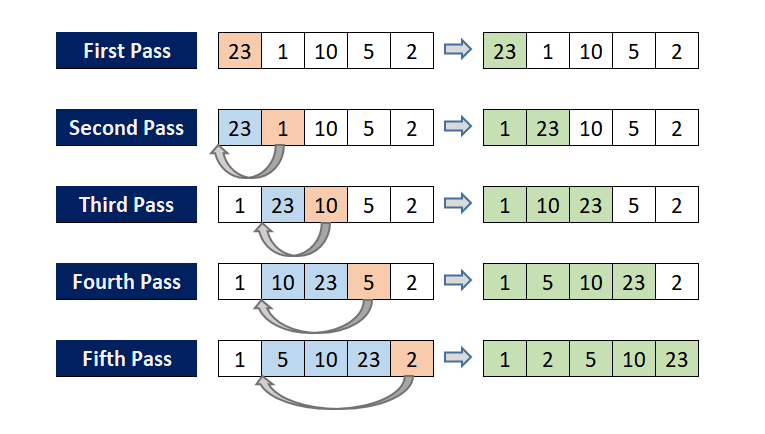
\includegraphics[scale=0.45]{ressources/insert.png}
        \caption{Exemple graphique d’un tri par insertion}
    \label{fig:insert}
\end{figure}
\\
\par
\begin{function}[H]
    \textbf{Variables :}\\
    i,j : entier\;
    tmp,longeur : entier\;
    
    
    \Begin{
        $longeur \leftarrow taille(T)$\;
        \For{$i \leftarrow 1$ \KwTo N-1}{
            $tmp \leftarrow tab[i]$\;
            $j\leftarrow i$\;
                   \While{$j>0$ et $tab[j-1]>tmp$} {
                     $tab[j] \leftarrow tab[j-1]$\;
                     $j \leftarrow j-1$\;
                   } 
            $tab[j] \leftarrow tmp$\;
        }
       
      
    }
    \caption{Insert(Entrée: tab: tableau d'entier; )}
\end{function}


\section{Calcul de complexité}
\subsection{Complexité temporelle}
\par
La complexité d’un algorithme de tri par insertion dépend de la taille n du tableau et de sa nature : si le tableau est déjà trié (ou partiellement trié), la complexité est en effet beaucoup moins important que si le tableau est trié dans l’ordre inverse.
\par
\textbf{Meilleur Cas :}
\par
Ce type de complexité se produit souvent lorsque les éléments du tableau initial sont triés.
 Il faut donc comparer un à un (n-1) éléments.
 \par
* La boucle (pour) s'exécute un nombre de fois égal à N-1.
\par
* la boucle (tant que)  ne s'exécute pas.

\par
Il y a donc N-1 comparaisons et au plus N affectations.
C(n)=N+(N-1)=2N+1.
La complexité du meilleur cas est d'ordre N. Il en résulte une complexité linéaire O(n).

\\
\textbf{Pire Cas :}
\par
Ce type de complexité se produit lorsque les éléments du tableau sont initialement triés dans l’ordre inverse.
\par
A chaque étape, tous les éléments du sous-tableau trié doivent donc être décalés vers la droite pour que l'élément à trier qui est plus petit que tous les éléments déjà triés à chaque étape puisse être placé au  début.
\par
Donc  on effectue l'échange a chaque comparaison.
\par
Le nombre d’échange est alors:
\par
C(n)=2+3+...+N-1= N(N-1)/2 .
\par
La complexité dans le pire des cas est d'ordre N^2. Il en résulte une complexité quadratique  O(n^2).
\par

\textbf{Moyen Cas :}
\par
Ce type de complexité se produit généralement lorsque les éléments d'un tableau sont mélangés de sorte que seulement la moitié des éléments sont décalé, ce qui signifie que chaque élément est plus petit que la moitié des éléments à sa gauche. En considérant un décalage de (p-1)/2 éléments, la complexité moyenne du calcul est donc :
C(n)=1/2+1+...+(N-1)/2= N(N-1)/4

La complexité sera donc la moitié de la complexité du pire cas, mais elle est toujours d'ordre N^{2}, donc c'est une complexité quadratique O(n^{2})


\subsection{Complexité spatiale}
Le tri par insertion englobe une complexité spatiale de O(1) en raison de l'utilisation d'une variable supplémentaire tmp.
\section{Experimentation}
Dans cette partie nous allons voir les résultats des exécutions de cet algorithme sur différents taille de tableau et sur données qui se représentent en 3 configuration ( triée en bon ordre , triée en ordre inverse , aléatoire) 
\subsubsection{Les données du tableau sont triées en bon ordre.}
\\
\begin{tabular}{| c | c | c | c | c | c | c | c | c | c | c |}
    \hline 
     Taille &  10000 & 50000 & 100000 & 500000 & 1000000 & 5000000 & 10000000 & 50000000 \\
    \hline
    temps(s) & 0.000014	& 0.000063 & 0.000136 &	0.000337	& 0.001291 &	0.003248 &	0.012637 &	0.064748	 \\
   \hline
   
\end{tabular}
\par

\subsubsection{Les données du tableau sont triées en ordre inverse.}
\\
\begin{tabular}{| c | c | c | c | c | c | c | c | c | c | c |}
    \hline 
     Taille &  10000 & 50000 & 100000 & 500000 & 1000000 & 5000000 & 10000000 & 50000000 \\
    \hline
    temps(s) & 0.061094 &	1.500352 &	6.068683 	& 101.321114 &	511.278107  &  & & \\
   
   \hline
\end{tabular}
\par
\subsubsection{Les données du tableau sont  positionnés aléatoirement.}
\\
\begin{tabular}{| c | c | c | c | c | c | c | c | c | c | c |}
    \hline 
     Taille &  10000 & 50000 & 100000 & 500000 & 1000000 & 5000000 & 10000000 & 50000000  \\
    \hline
    temps(s) & 0.017770 &	0.537932 & 1.994625	 & 60.600109 &	223.830612 &  & &\\
    \hline
   
   
\end{tabular}
\par
\subsubsection{Le graphe :}
\\
La figure suivante représente les résultats d'exécution de cet algorithme selon les différentes taille du tableau.
\\
\begin{figure}[H]
    \centering
        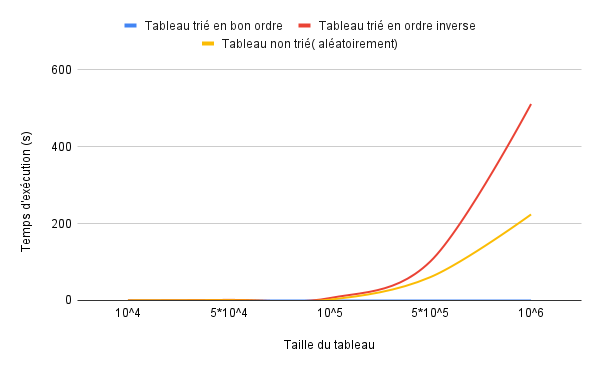
\includegraphics[scale=0.7]{ressources/ChartInsert.png}
        \caption{Temps d'execution du tri par insertion sur les différents taille du tableau }
    \label{fig:insertch}
\end{figure}
\\
D’après le graphique et les tableaux ci-dessus, nous remarquons que le tri par insertion prend beaucoup de temps lors du tri des éléments dans l'ordre inverse ou dans leur positionnement aléatoire, Les courbes s‘évoluent d’une manière quadratique à chaque fois que la taille du tableau augmente. Cependant, si les éléments sont déjà triés, cela fonctionne très bien et ne prend pas beaucoup de temps. 
\par
On en conclut que la complexité théorique est cohérente avec les résultats expérimentaux.

\section{Conclusion}
A partir d'étude expérimentale et théorique de l'algorithme tri par insertion, On constate que malgré sa complexité en temps quadratique sur des données inversées ou triées aléatoirement, il est encore largement utilisé car il est capable de s'exécuter en temps linéaire sur des entrées déjà triées, et de manière très efficace sur de petites entrées.

